\subsubsection{Feature}
\label{sec:Feature}

The \sbol{Feature} class, as shown in \ref{uml:subcomponent} is used to compose \sbol{Component} objects into a structural or functional hierarchy. 

\begin{figure}[ht]
\begin{center}
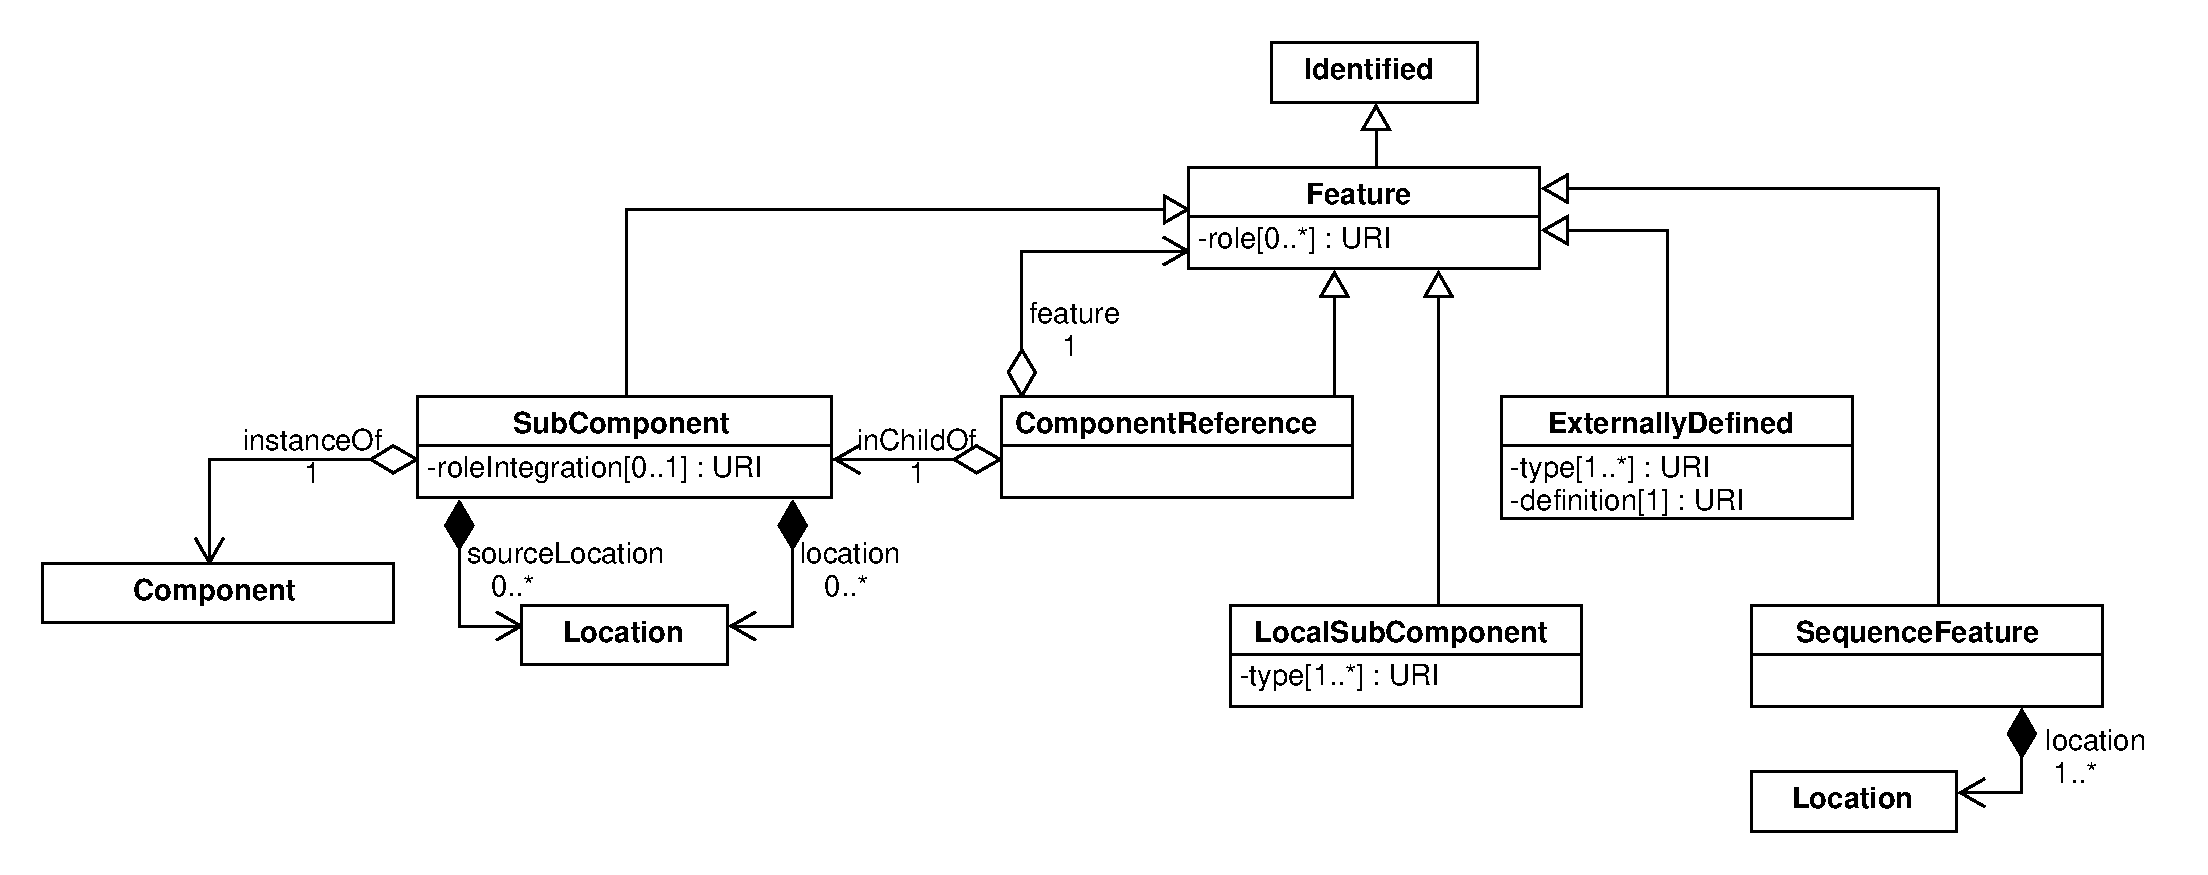
\includegraphics[width=\textwidth]{uml/feature}
\caption[]{Diagram of the \sbol{Feature} class and its associated properties.}
\label{uml:subcomponent}
\end{center}
\end{figure}

\subparagraph{The \sbolheading{role} property}\label{sec:roles:C}

The expected purpose and function of a genetic part are described by the
\sbolmult{roles:CD}{roles} property of \sbol{Component}. However, the same building block might be used for a different purpose in an actual design. In other words, purpose and function are sometimes determined by context. 

The \sbolmult{roles:C}{roles} property comprises an OPTIONAL set of zero or more \sbolmult{roles:C}{role} \sbol{URI}s describing the purpose or potential function of this \sbol{Feature}'s included sub-\sbol{Component} in the \textit{context} of its parent \sbol{Component}.
If provided, these \sbolmult{roles:C}{role} \sbol{URI}s MUST identify terms from appropriate ontologies. Roles are not restricted to describing biological function; they may annotate a \sbol{Feature}'s function in any domain for which an ontology exists.

It is RECOMMENDED that these \sbolmult{roles:C}{role} \sbol{URI}s identify terms that are compatible with the \sbolmult{types:CD}{type} properties of both this \sbol{Feature}'s parent \sbol{Component} and its included sub-\sbol{Component}. For example, a \sbolmult{roles:C}{role} of a \sbol{Feature} which belongs to a \sbol{Component} of type DNA and includes a sub-\sbol{Component} of type DNA might refer to terms from the Sequence Ontology. A table of recommended ontology terms for \sbolmult{roles:C}{roles} is given in \ref{tbl:component_roles}.

\paragraph{SubComponent}
\label{sec:SubComponent}

The \sbol{SubComponent} class a subclass of the \sbol{Feature} class that can be used to specify structural hierarchy. For example, the \sbol{Component} of a gene could contain four \sbol{SubComponent} objects: a promoter, RBS, CDS, and terminator. In turn, the \sbol{Component} of the promoter \sbol{SubComponent} could contain \sbol{SubComponent} objects defined as various operator sites.

\subparagraph{The \sbolheading{roleIntegration} property}\label{sec:roleIntegration:C}


A \sbolmult{roleIntegration:C}{roleIntegration} specifies the relationship between a \sbol{Feature} instance's own set of \sbolmult{roles:C}{roles} and the set of \sbolmult{roles:CD}{roles} on the included sub-\sbol{Component}.

The \sbolmult{roleIntegration:C}{roleIntegration} property has a data type of \sbol{URI}. A \sbol{Feature} instance with zero \sbolmult{roles:C}{roles} MAY OPTIONALLY specify a \sbolmult{roleIntegration:C}{roleIntegration}. A \sbol{Feature} instance with one or more \sbolmult{roles:C}{roles} MUST specify a \sbolmult{roleIntegration:C}{roleIntegration} from \ref{tbl:component_roleIntegration}.
If zero \sbol{Feature} \sbolmult{roles:C}{roles} are given and no \sbol{Feature} \sbolmult{roleIntegration:C}{roleIntegration} is given, then \url{http://sbols.org/v2\#mergeRoles} is assumed.
It is RECOMMENDED to specify a set of \sbol{Feature} \sbolmult{roles:C}{roles} only if the integrated result set of roles would differ from the set of \sbolmult{roles:CD}{roles} belonging to this \sbol{Feature}'s included sub-\sbol{Component}.


\begin{table}[ht]
  \begin{edtable}{tabular}{lp{4in}}
    \toprule
    \textbf{roleIntegration URI} & \textbf{Description} \\
    \midrule
    \url{http://sbols.org/v2\#overrideRoles} & In the context of this \sbol{Feature}, ignore any \sbolmult{roles:CD}{roles} given for the included sub-\sbol{Component}. Instead use only the set of zero or more \sbolmult{roles:C}{roles} given for this \sbol{Feature}. \\
    \url{http://sbols.org/v2\#mergeRoles} & Use the union of the two sets: both the set of zero or more \sbolmult{roles:C}{roles} given for this \sbol{Feature} as well as the set of zero or more \sbolmult{roles:CD}{roles} given for the included sub-\sbol{Component}. \\
    \bottomrule
  \end{edtable}
  \caption{Each \sbolmult{roleIntegration:C}{roleIntegration} mode is associated with a rule governing how a \sbol{Feature}'s roles are to be combined with the included 
sub-\sbol{Component}'s roles.}
  \label{tbl:component_roleIntegration}
\end{table}


\subparagraph{The \sbolheading{instanceOf} property}
\label{sec:instanceOf}

The \sbol{instanceOf} property is a REQUIRED \sbol{URI} that refers to the \sbol{Component} of the \sbol{Feature}.
As described in the previous section, this \sbol{Component} effectively provides information about the \sbolmult{types:CD}{types} and \sbolmult{roles:CD}{roles} of the \sbol{Feature}.

The \sbol{instanceOf} property MUST NOT refer to the same \sbol{Component} as the one that contains the \sbol{Feature}.
Furthermore, \sbol{Feature} objects MUST NOT form a cyclical chain of references via their \sbol{instanceOf} properties and the \sbol{Component} objects that contain them.
For example, consider the \sbol{Feature} objects $A$ and $B$ and the \sbol{Component} objects $X$ and $Y$. The reference chain ``$X$ contains $A$, $A$ is defined by $Y$, $Y$ contains $B$, and $B$ is defined by $X$'' is cyclical.

The \sbol{sourceLocations} property is an OPTIONAL set of zero or more \sbol{Location} objects that indicate which \sbol{elements} of a \sbol{Component}'s \sbol{Sequence} are to be included in the \sbol{Component}'s parent. The \sbol{sourceLocations} property
allows for only a portion of a \sbol{Component}'s \sbol{Sequence} to be included, rather than its entirety.

If the \sbol{sourceLocation} property is not set, then the whole \sbol{Sequence} is assumed to be included. Alternatively,
if the \sbol{sourceLocation} property is set, then the relationship between the original \sbol{Component}'s
\sbol{Sequence} and the included \sbol{Sequence} is defined identically to the \sbol{locations}
property on the \sbol{SequenceFeature} object.


\subparagraph{The \sbolheading{location} property}\label{sec:location}
The \sbol{location} property is an OPTIONAL set which points to a \sbol{Location} on the parent \sbol{Component} sequence; if \sbol{location} is missing, this indicates a part / sub-part relationship for which sequence details have not (yet) been determined.

The \sbol{Location} record(s) specified by a \sbol{Feature} are subject to the same restrictions currently in place for \sbol{SequenceFeature} \sbol{Location}. Concretely, two \sbol{Location} records attached to the same \sbol{Feature} MUST NOT overlap in their range as it would not be clear what that means. The \sbol{Location} of two separate \sbol{Feature}s may overlap.

\subparagraph{The \sbolheading{orientation} property}\label{sec:orientation2}
The \sbol{orientation} property is OPTIONAL and has a data type of \sbol{URI}. All subclasses of \sbol{Feature} share this property, which can be used to indicate how the region specified by the \sbol{SequenceFeature} and any associated double-stranded \sbol{SubComponent} is oriented on the \sbol{elements} of a \sbol{Sequence}  from their parent \sbol{Component}. \ref{tbl:orientation_types} provides a list of REQUIRED \sbol{orientation} \sbol{URI}s. If a \sbol{Feature} object has an \sbol{orientation}, then it MUST come from \ref{tbl:orientation_types}.

\todo{add best practice here talking about EntireComponent?}


\paragraph{ComponentReference}
\label{sec:ComponentReference}

The \sbol{ComponentReference} class is a subclass of \sbol{Feature} and a sibling of the \sbol{SubComponent} class. 


\subparagraph{The \sbolheading{inChildOf} property}\label{sec:inChildOf}

The \sbol{inChildOf} property is a REQUIRED \sbol{URI} that refers to a SubComponent. \sbol{inChildOf} must refer to a \sbol{SubComponent} pointed directly to by the parent of the \sbol{ComponentReference} (i.e., as a \sbol{SubComponent} of \sbol{Component}, or an \sbol{inChildOf} of \sbol{ComponentReference}). If the \sbol{Feature} is a \sbol{SubComponent}, then it must be a child of the \sbol{SubComponent} pointed to by \sbol{inChildOf}.

\subparagraph{The \sbolheading{feature} property}\label{sec:feature:CR}

The \sbolmult{feature:CR}{feature} property is an OPTIONAL \sbol{URI} that refers to a \sbol{Feature}.

\paragraph{LocalSubComponent}
\label{sec:LocalSubComponent}

The \sbol{LocalSubComponent} class a subclass of \sbol{Feature}. This class was serves as a way to create an ``empty'' \sbol{Component} to serve as a placeholder in more complex \sbol{Component}s. 

\subparagraph{The \sbolheading{type} property}\label{sec:type:LSC}

The \sbolmult{type:LSC}{type} property is REQUIRED and contains one or more \sbol{URI}s. The \sbolmult{type:LSC}{type} property is identical to its use in \sbol{Component}

\paragraph{ExternallyDefined}
\label{sec:ExternallyDefined}

The \sbol{ExternallyDefined} class has been introduced so that external definitions in databases like CHEBI or UniProt can be referenced.

\subparagraph{The \sbolheading{type} property}\label{sec:type:ED}

The \sbolmult{type:ED}{type} property is REQUIRED and contains one or more \sbol{URI}s. The \sbolmult{type:ED}{type} property is identical to its use in \sbol{Component}

\subparagraph{The \sbolheading{definition} property}\label{sec:definition:ER}

The \sbolmult{definition:ER}{definition} property is REQUIRED and contains one \sbol{URI} that links to a cononical definition external to SBOL.


\paragraph{SequenceFeature}
\label{sec:SequenceFeature}

The \sbol{SequenceFeature} class describes one or more regions of interest on the \sbol{Sequence} objects referred to by its parent \sbol{Component}. 
%In addition, \sbol{SequenceFeature} objects can describe the substructure of their parent \sbol{Component} through association with the \sbol{Feature} objects contained by this \sbol{Component}.

\subparagraph{The \sbolheading{locations} property}\label{sec:locations}
The \sbol{locations} property is a REQUIRED set of one or more \sbol{Location} objects that indicate which \sbol{elements} of a \sbol{Sequence} are described by the \sbol{SequenceFeature}.

Allowing multiple \sbol{Location} objects on a single \sbol{SequenceFeature} is intended to enable representation of discontinuous regions (for example, a \sbol{Feature} encoded across a set of exons with interspersed introns).
As such, the \sbol{Location} objects of a single \sbol{SequenceFeature} SHOULD NOT specify overlapping regions, since it is not clear what this would mean.
There is no such concern with different \sbol{SequenceFeature} objects, however, which can freely overlap in \sbol{Location} (for example, specifying overlapping linkers for sequence assembly).
